\section{Anhang}
\begin{figure}[h]
\begin{center}
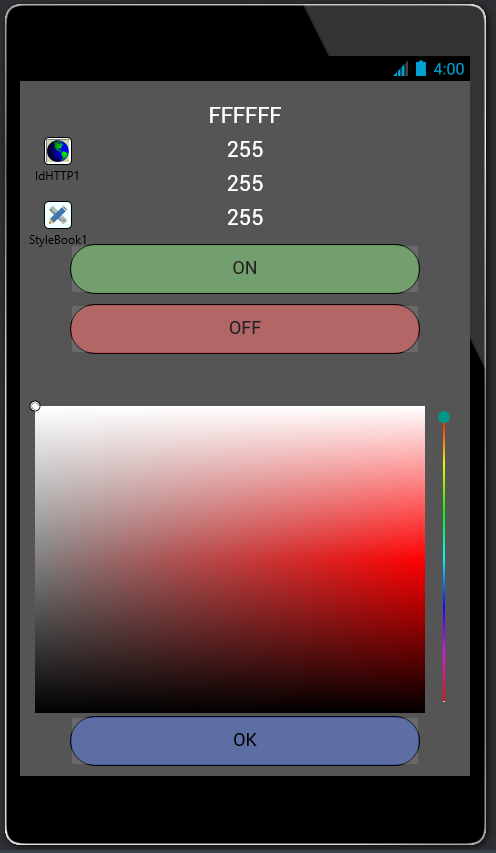
\includegraphics[width=8cm]{img/entwurf.png}
\caption{Entwurf}
\label{entwurf}
\end{center}
\end{figure}

\begin{figure}[h]
\begin{center}
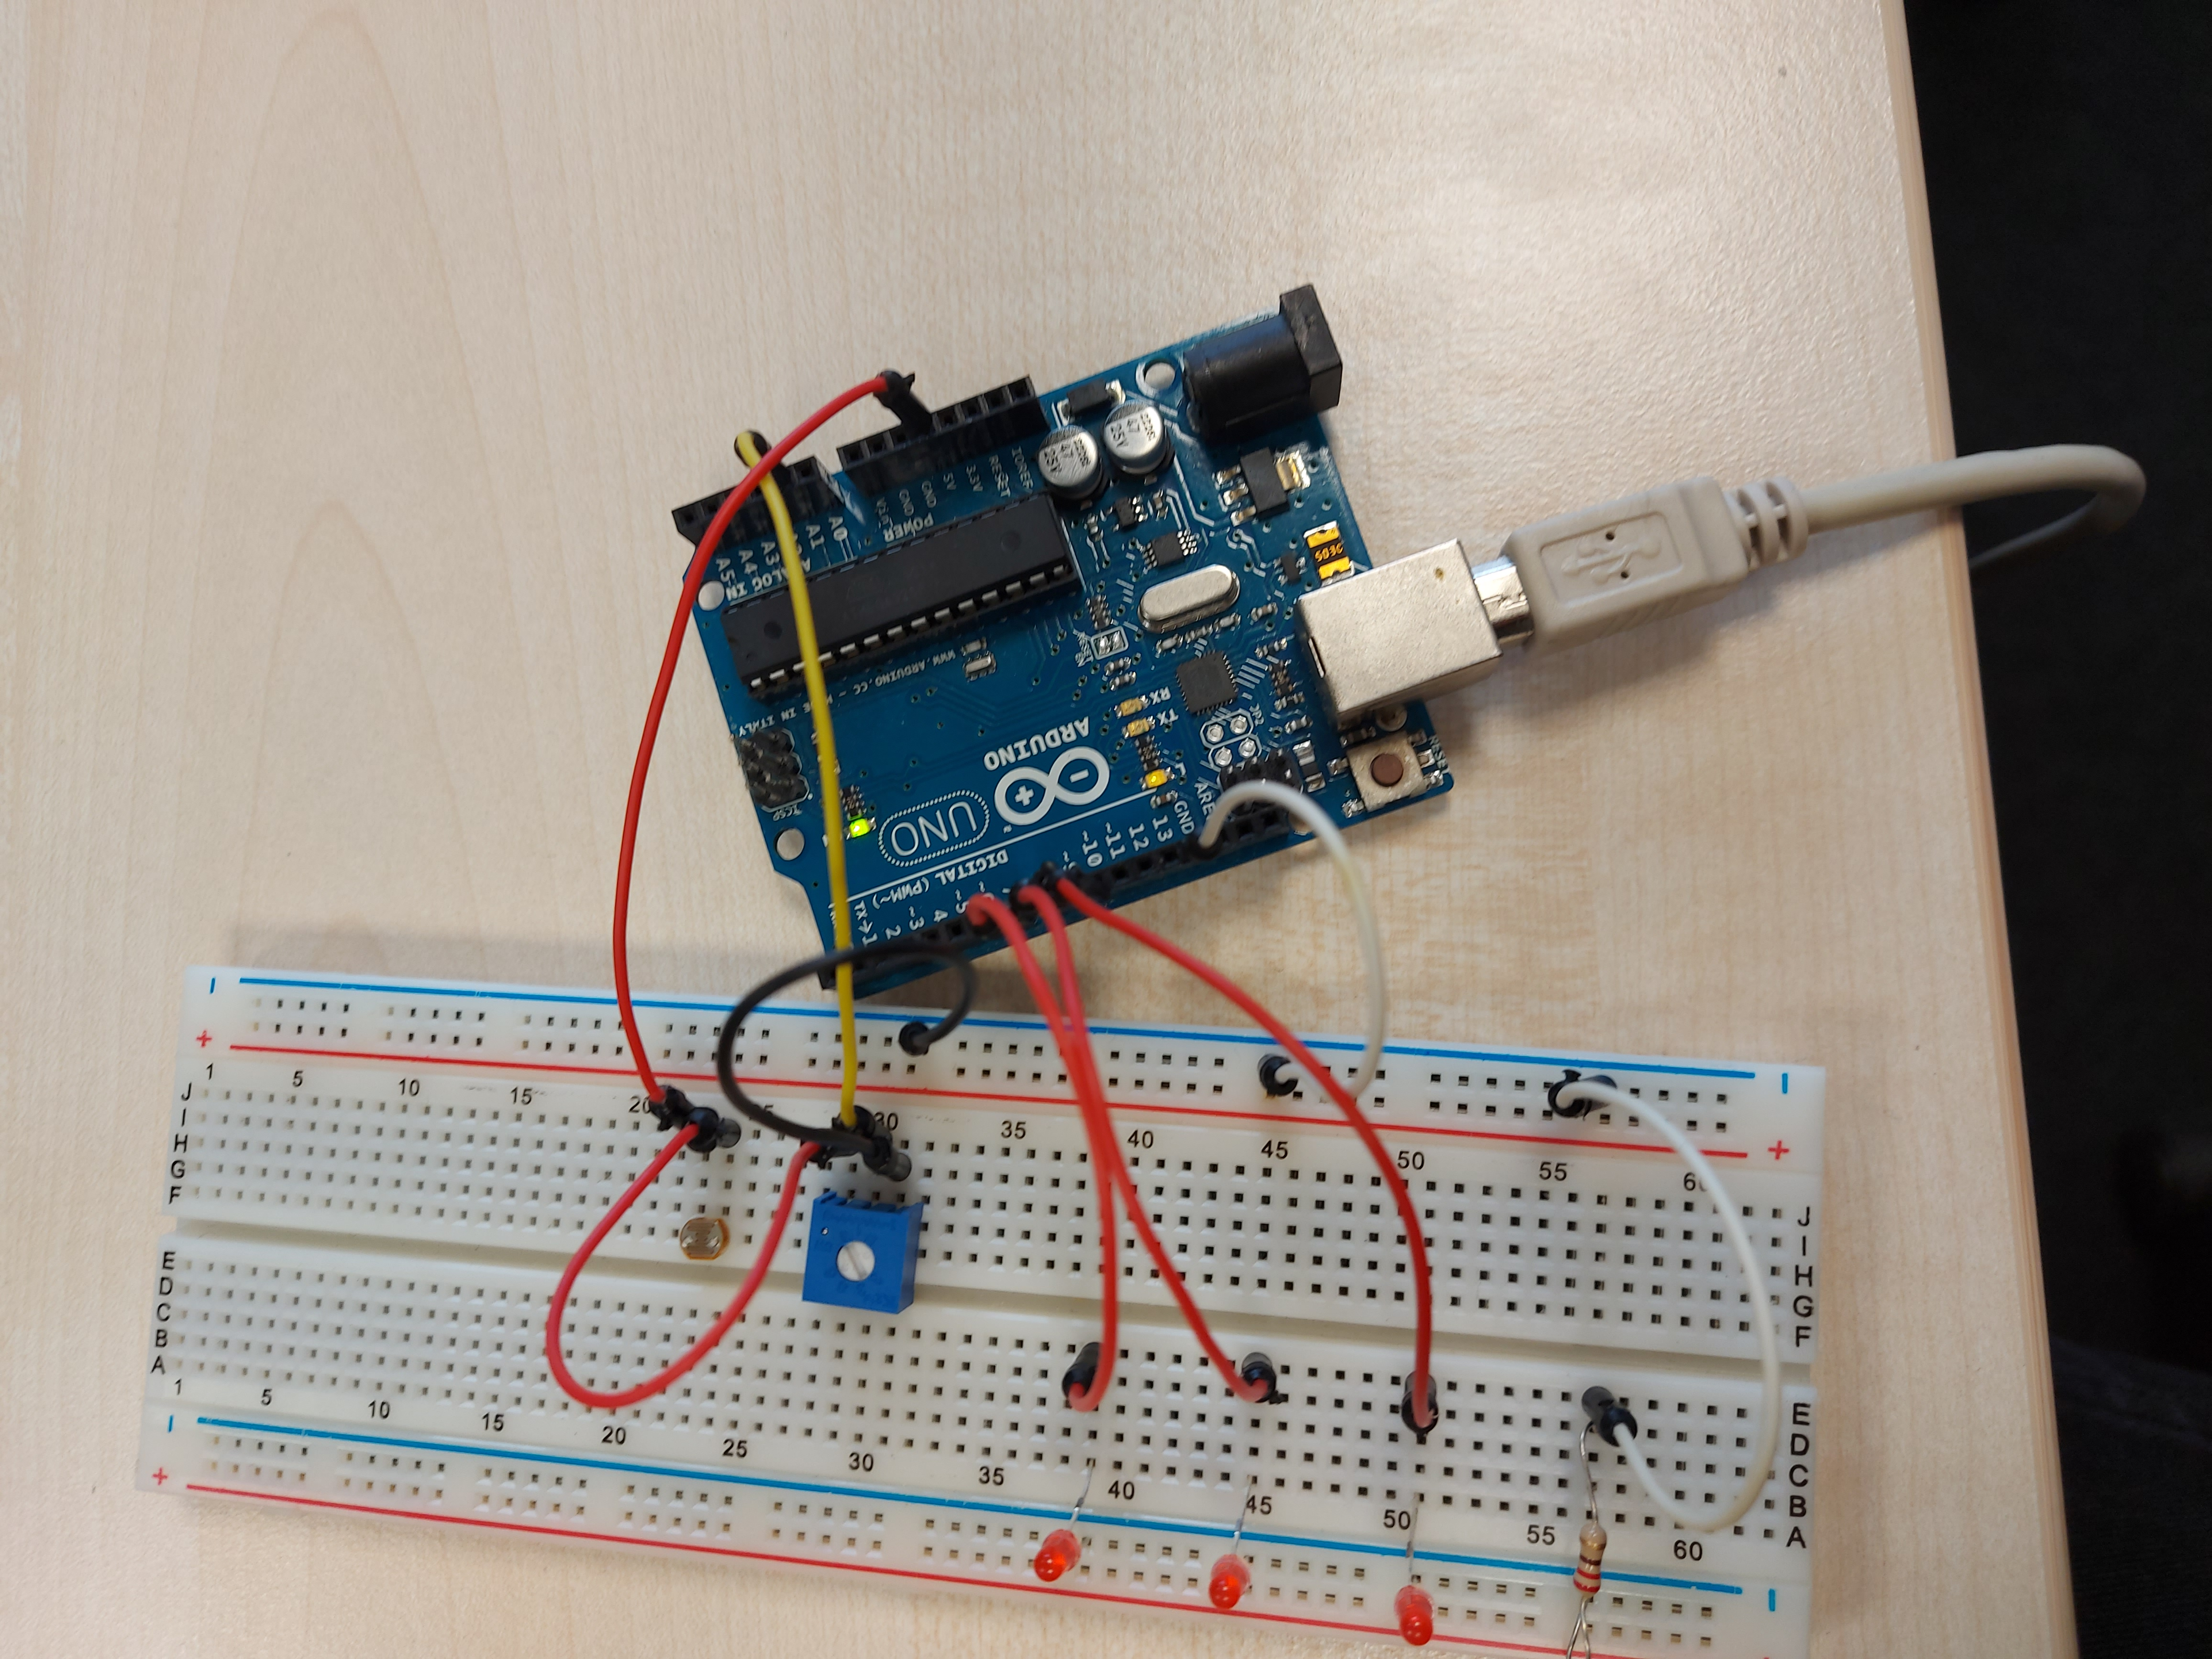
\includegraphics[width=15cm]{img/esp32testled.jpg}
\caption{Arduino Test Led Aufbau}
\label{esp32testled}
\end{center}
\end{figure}

\begin{figure}[h]
\begin{center}
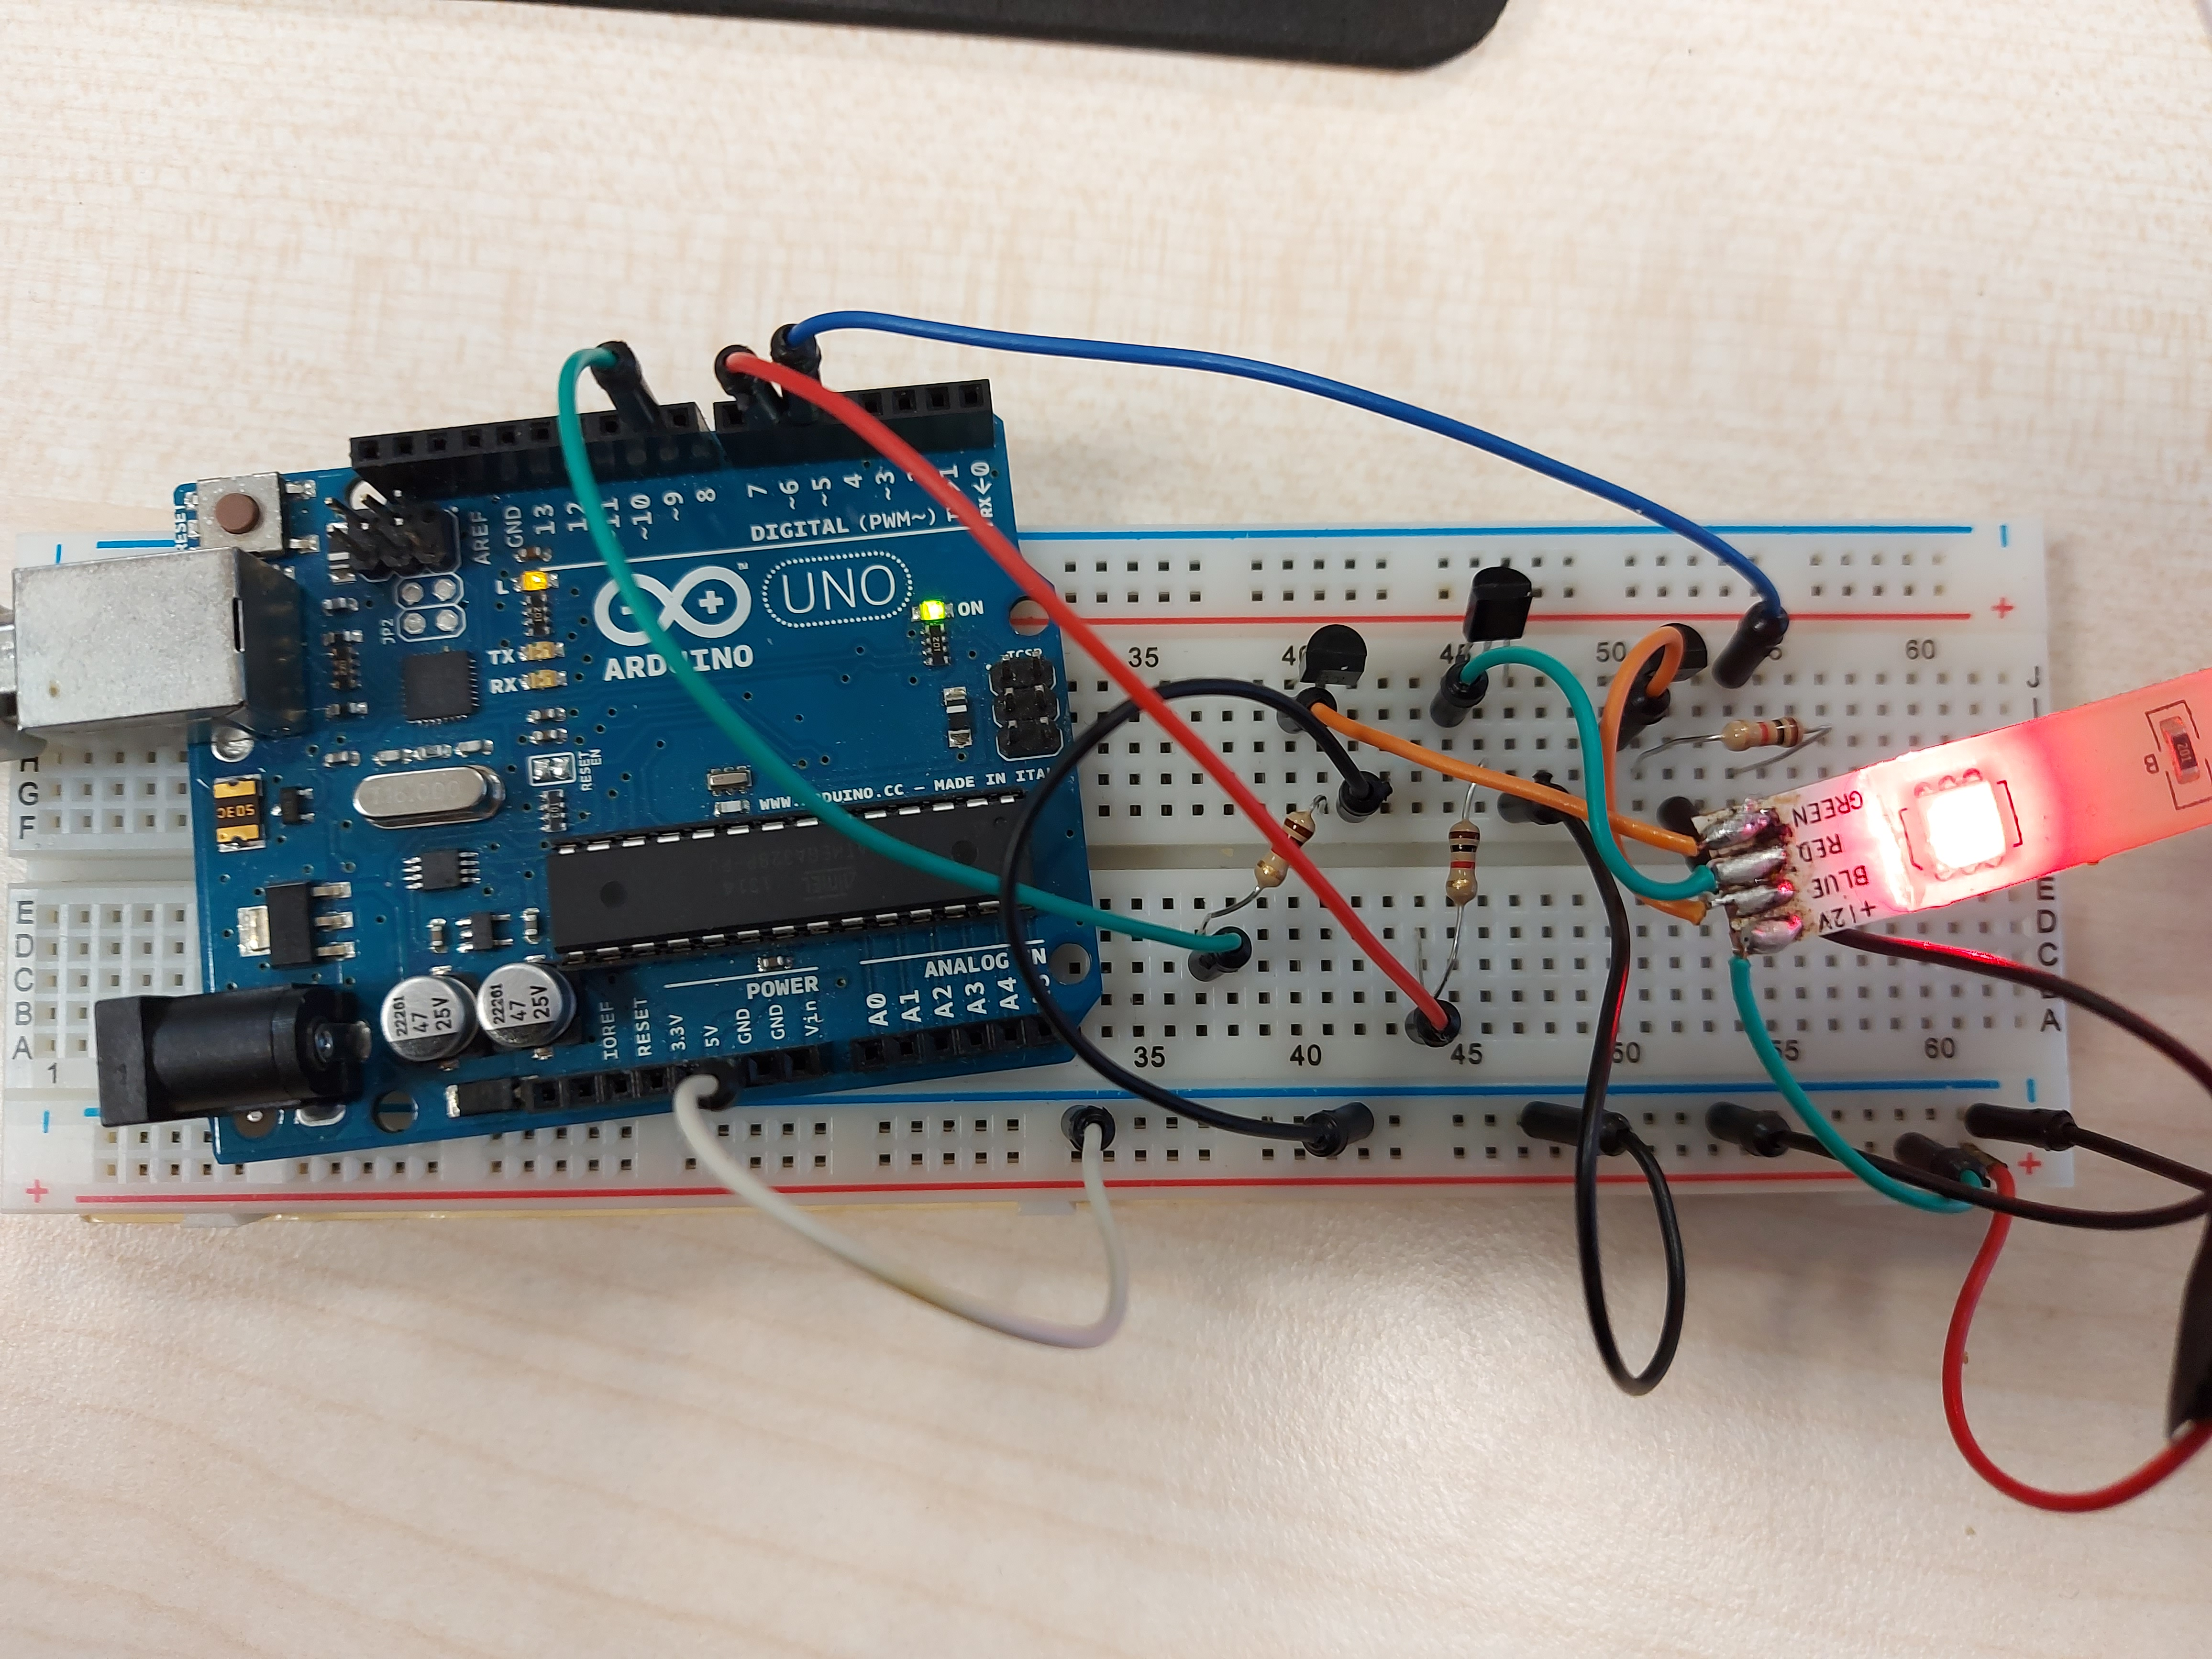
\includegraphics[width=15cm]{img/arduinoaufbau.jpg}
\caption{Arduino Aufbau}
\label{arduinoaufbau}
\end{center}
\end{figure}

\begin{figure}[h]
\begin{center}
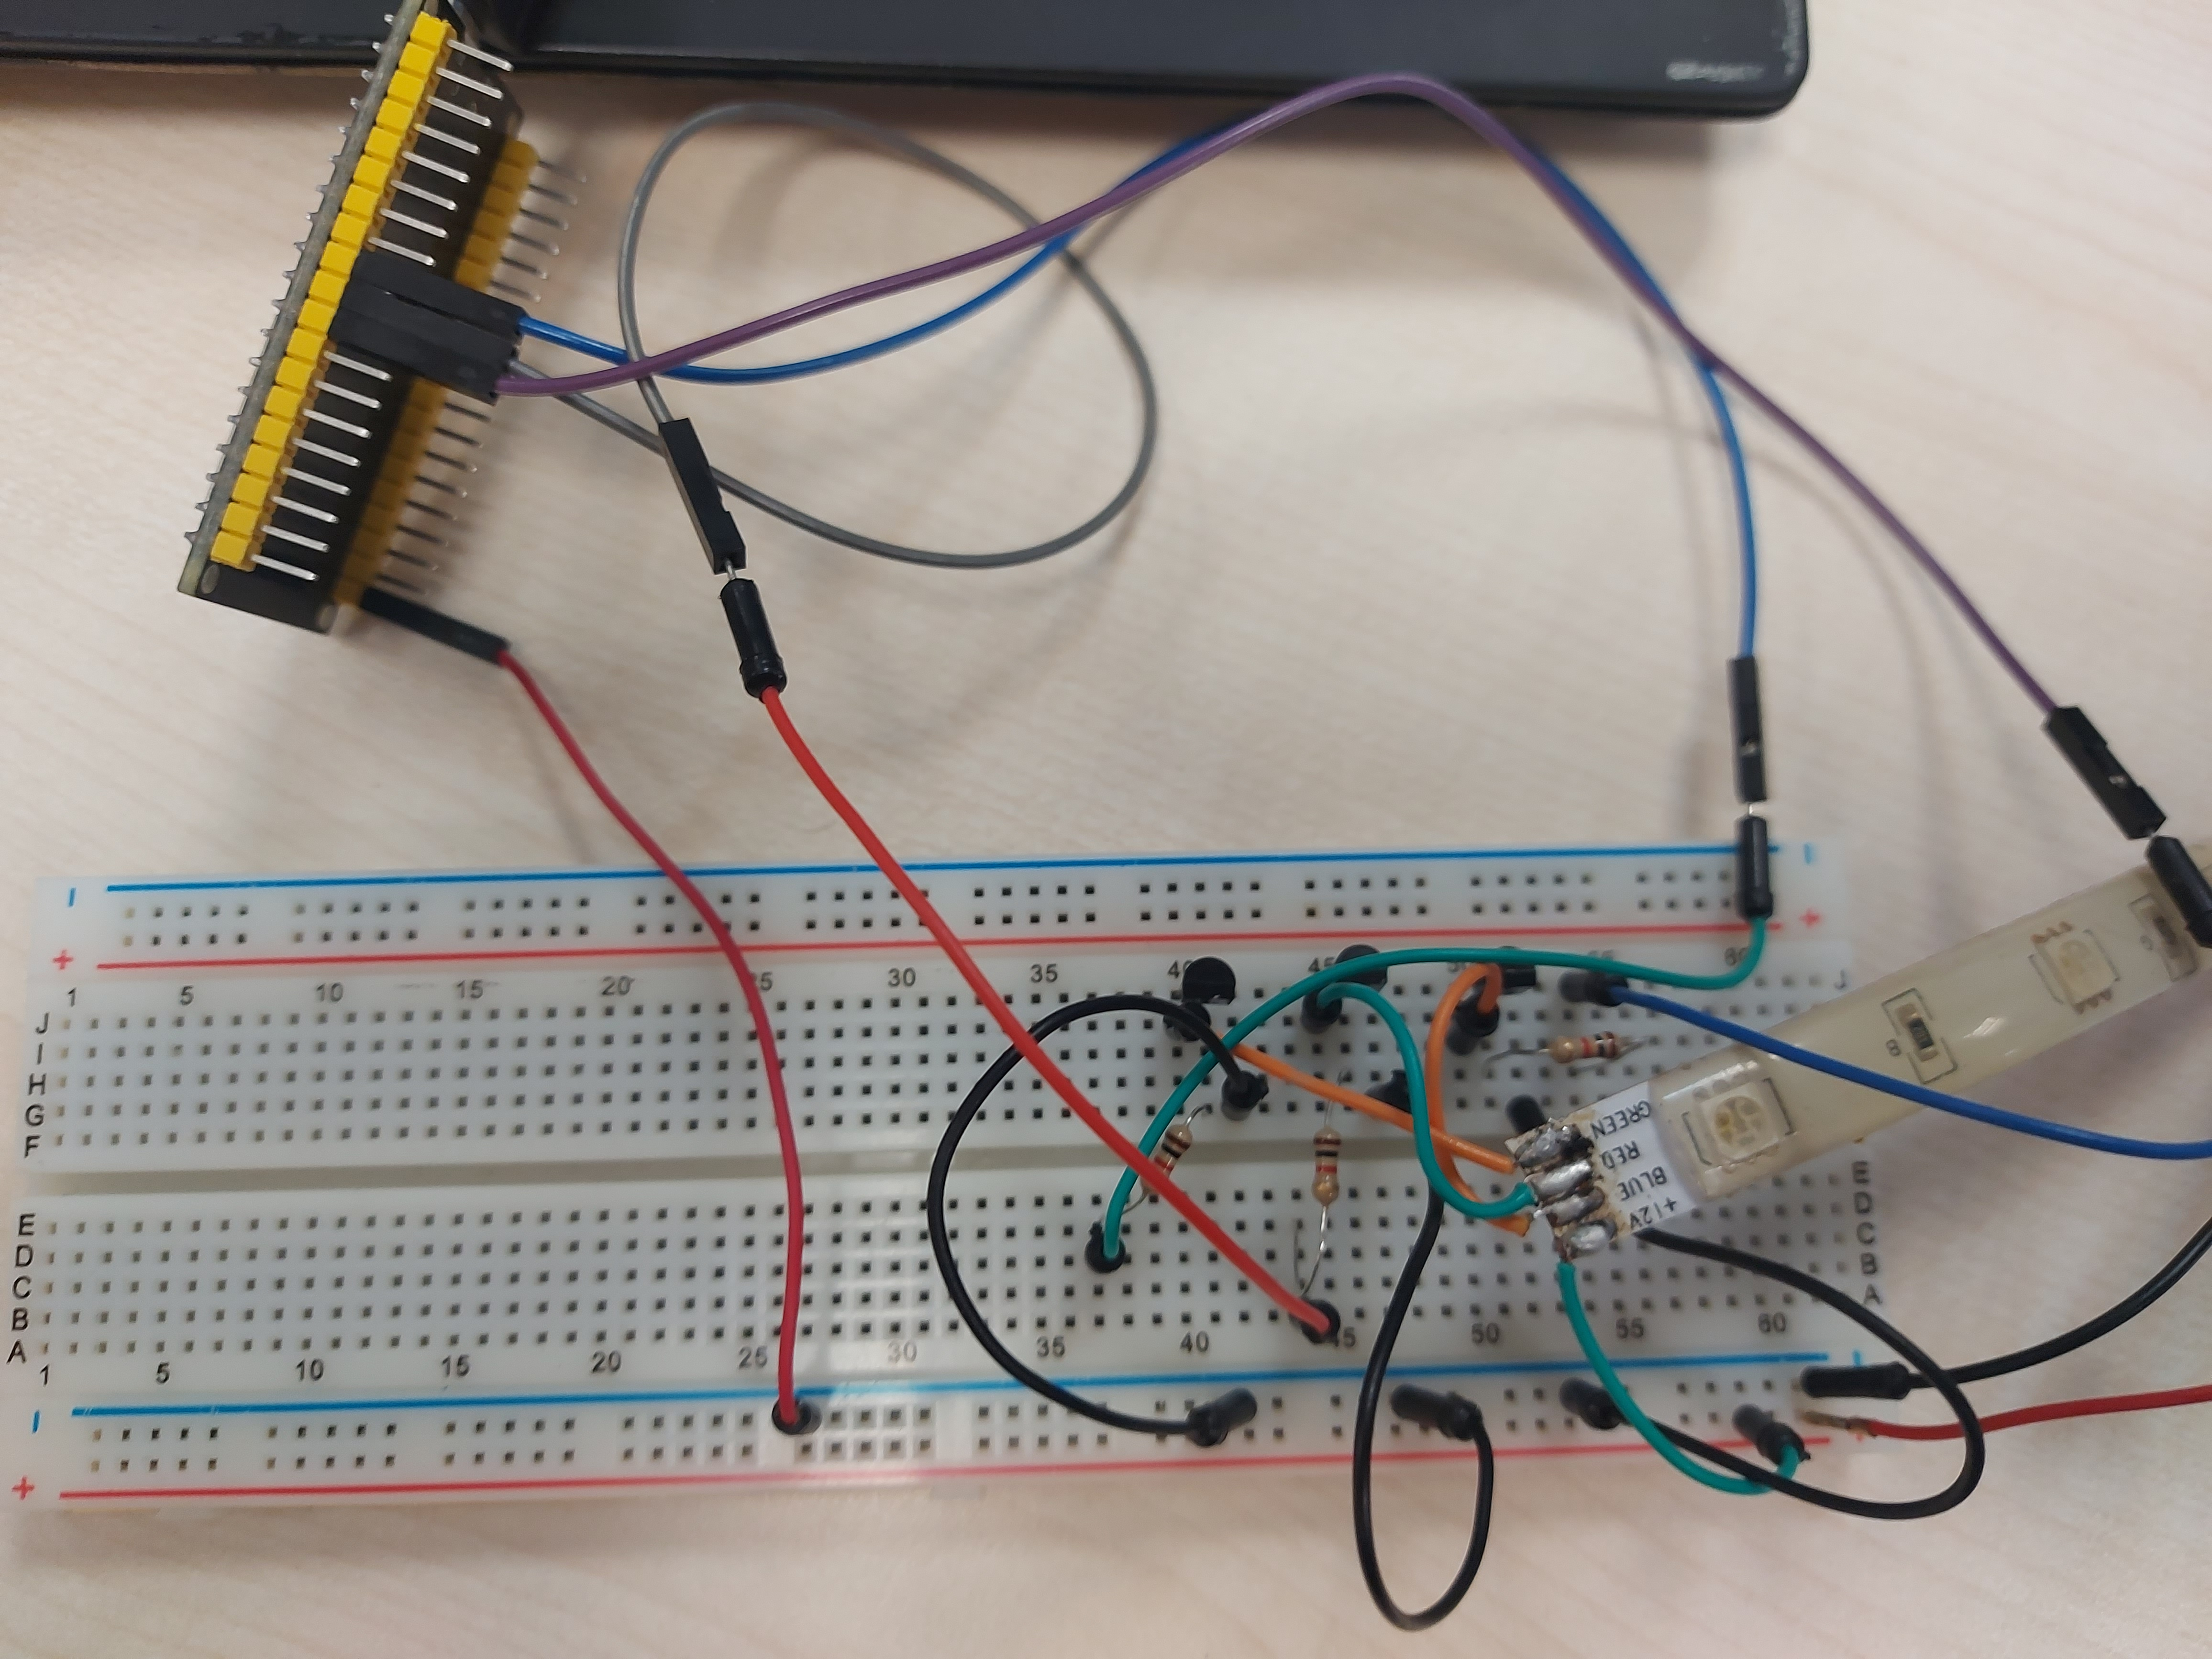
\includegraphics[width=15cm]{img/esp32aufbau.jpg}
\caption{ESP-32 Aufbau}
\label{esp32aufbau}
\end{center}
\end{figure}

\begin{figure}[h]
\begin{center}
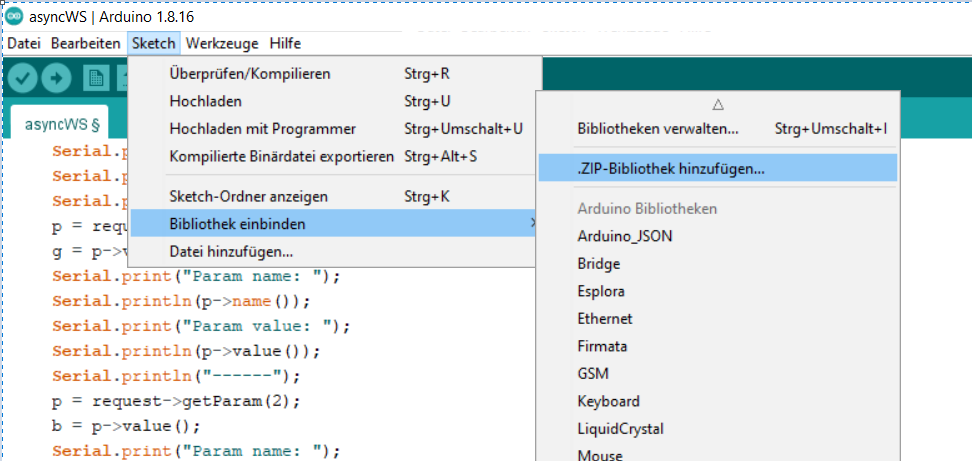
\includegraphics[width=15cm]{img/arduinosetup1.png}
\caption{Setup Arduino}
\label{arduinosetup1}
\end{center}
\end{figure}

\begin{figure}[h]
\begin{center}
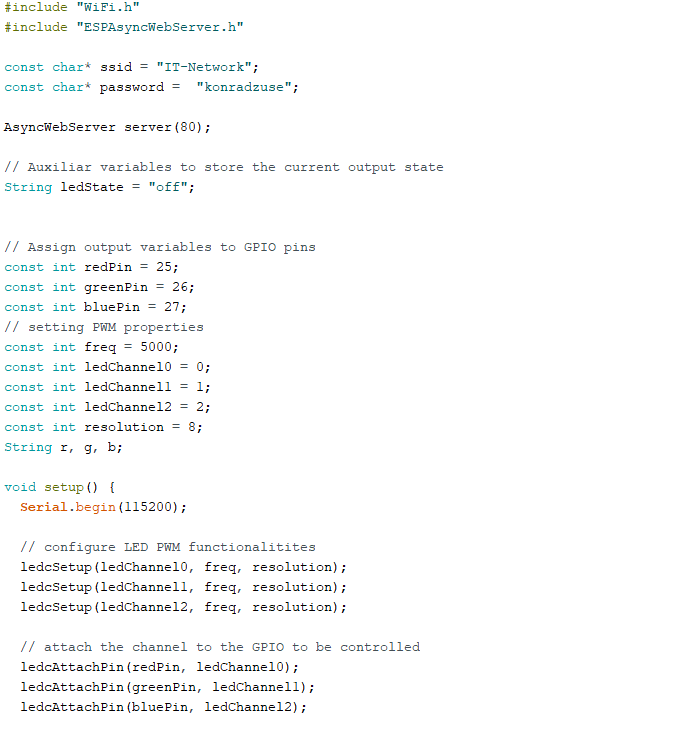
\includegraphics[width=15cm]{img/arduinocode1.png}
\caption{Arduino Code 1}
\label{arduinocode1}
\end{center}
\end{figure}

\begin{figure}[h]
\begin{center}
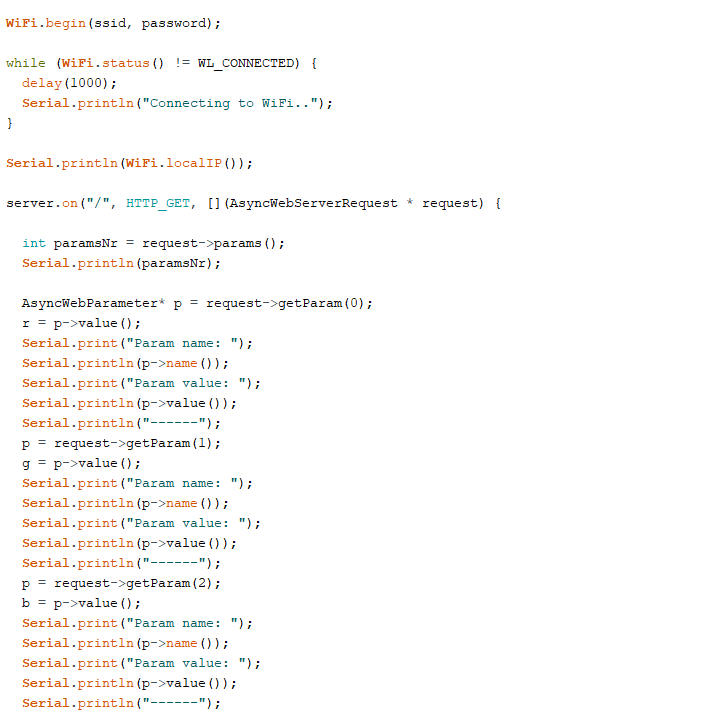
\includegraphics[width=15cm]{img/arduinocode2.png}
\caption{Arduino Code 2}
\label{arduinocode2}
\end{center}
\end{figure}

\begin{figure}[h]
\begin{center}
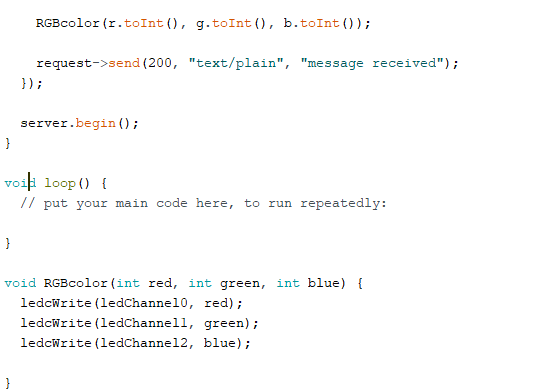
\includegraphics[width=15cm]{img/arduinocode3.png}
\caption{Arduino Code 3}
\label{arduinocode3}
\end{center}
\end{figure}

\begin{figure}[h]
\begin{center}
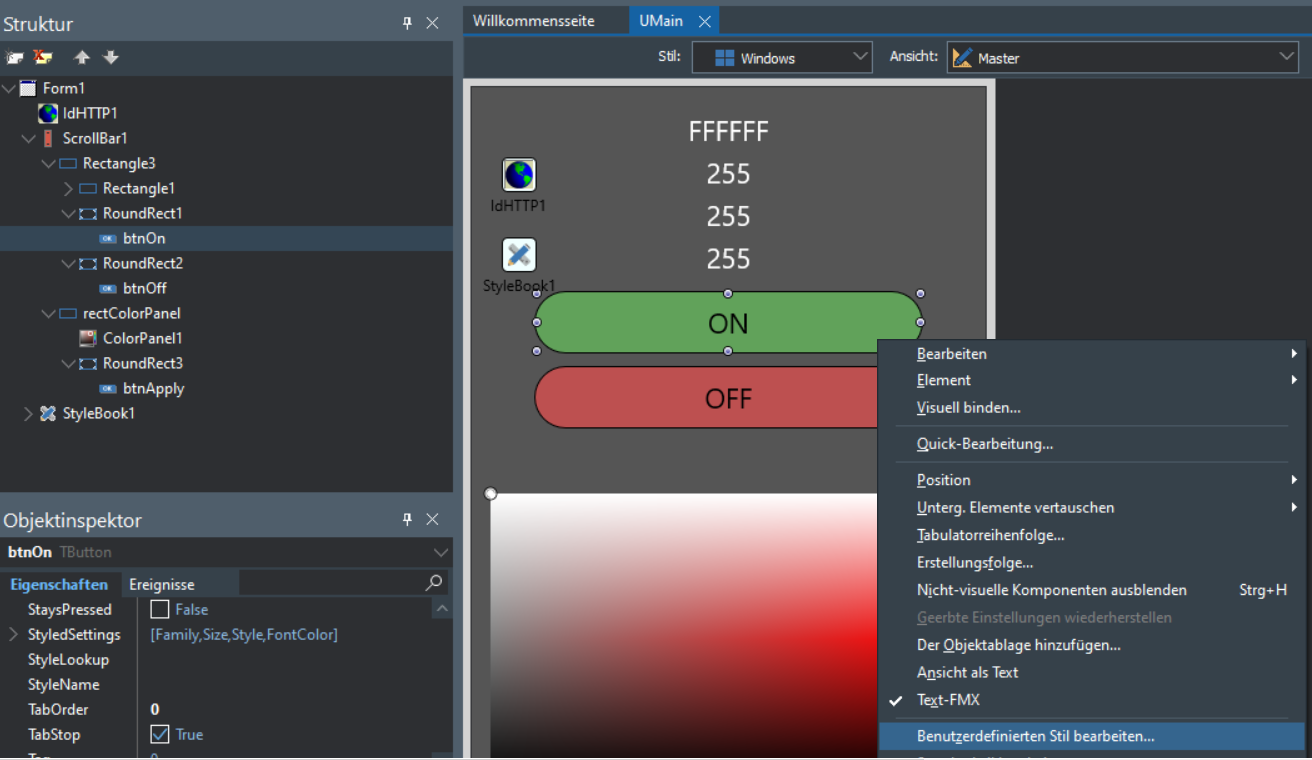
\includegraphics[width=15cm]{img/designstrucktur.png}
\caption{Design Struktur}
\label{designstruktur}
\end{center}
\end{figure}

\begin{figure}[h]
\begin{center}
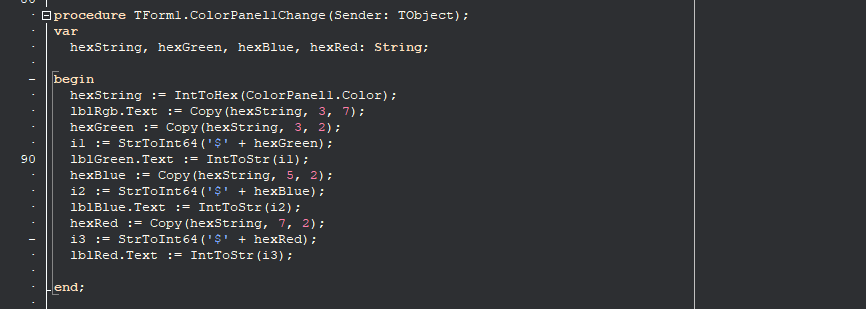
\includegraphics[width=15cm]{img/colorchange.png}
\caption{Das Color Change Event}
\label{colorchange}
\end{center}
\end{figure}

\begin{figure}[h]
\begin{center}
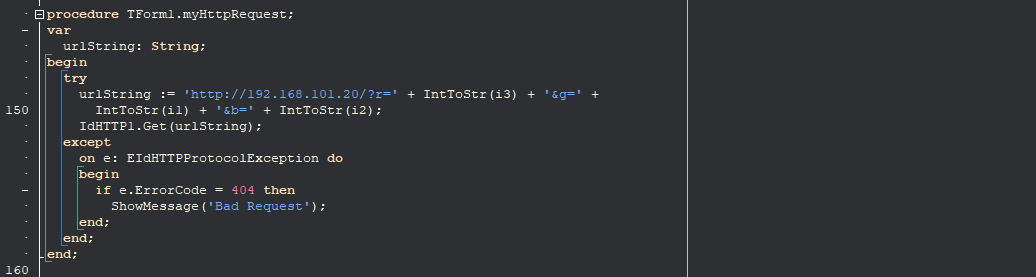
\includegraphics[width=15cm]{img/httprequest.png}
\caption{Der HTTP Request}
\label{httprequest}
\end{center}
\end{figure}

\begin{figure}[h]
\begin{center}
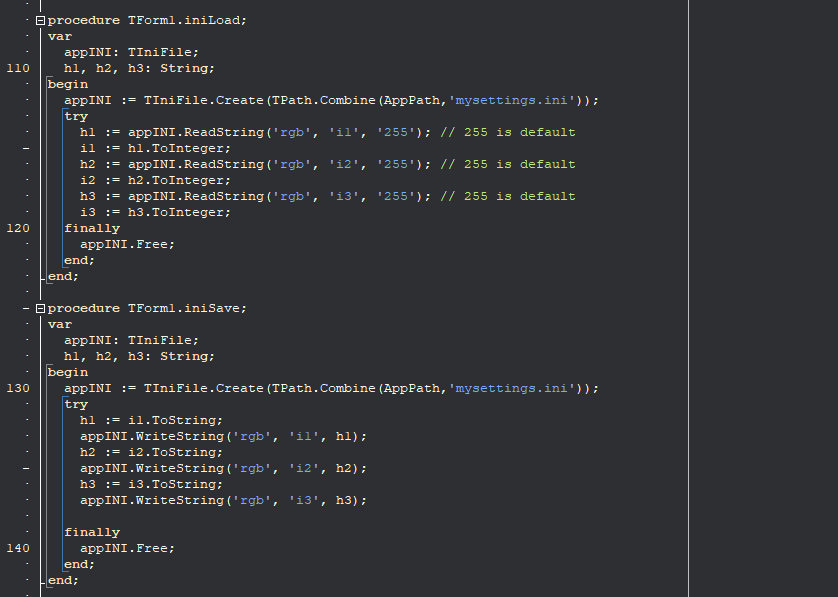
\includegraphics[width=15cm]{img/iniloadsave.png}
\caption{Die Methoden iniload und inisave}
\label{iniloadsave}
\end{center}
\end{figure}

\begin{figure}[h]
\begin{center}
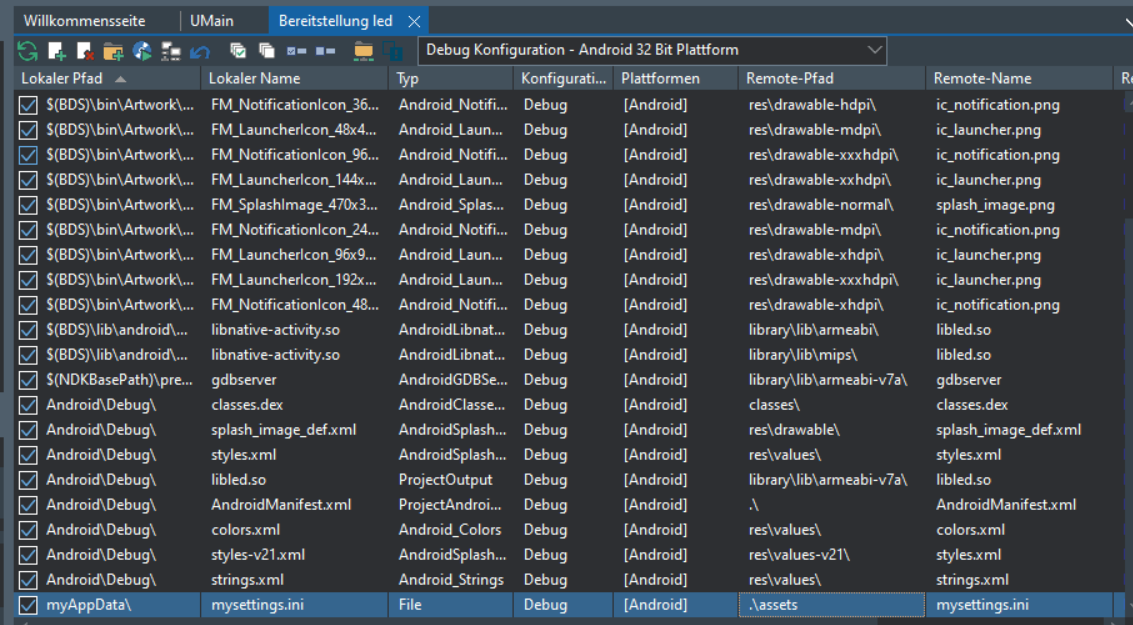
\includegraphics[width=15cm]{img/bereitstellung.png}
\caption{Die Bereitstellung der ini für Android}
\label{bereitstellung}
\end{center}
\end{figure}

\begin{figure}[h]
\begin{center}
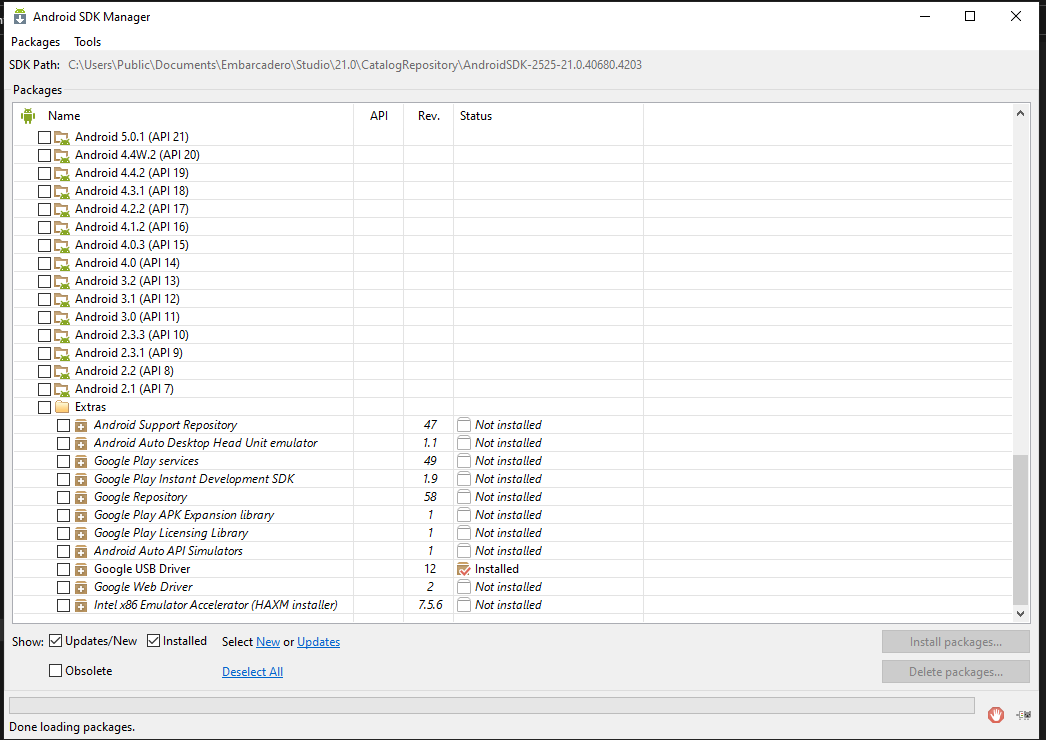
\includegraphics[width=15cm]{img/sdkmanager.png}
\caption{Der SDK Manager}
\label{sdkmanager}
\end{center}
\end{figure}

\begin{figure}[h]
\begin{center}
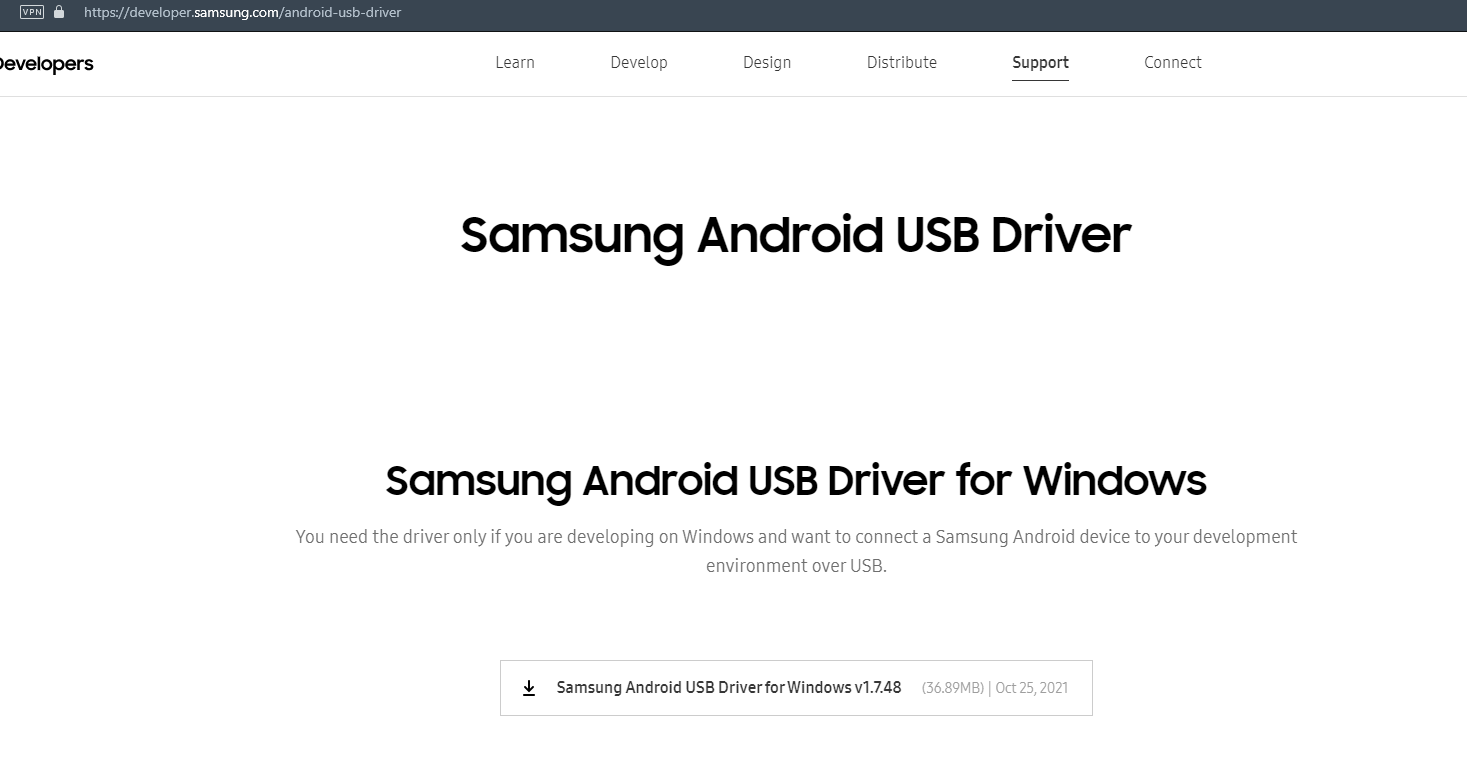
\includegraphics[width=15cm]{img/samsungusb.png}
\caption{USB Treiber für Samsung Android}
\label{samsungusb}
\end{center}
\end{figure}

\begin{figure}[h]
\begin{center}
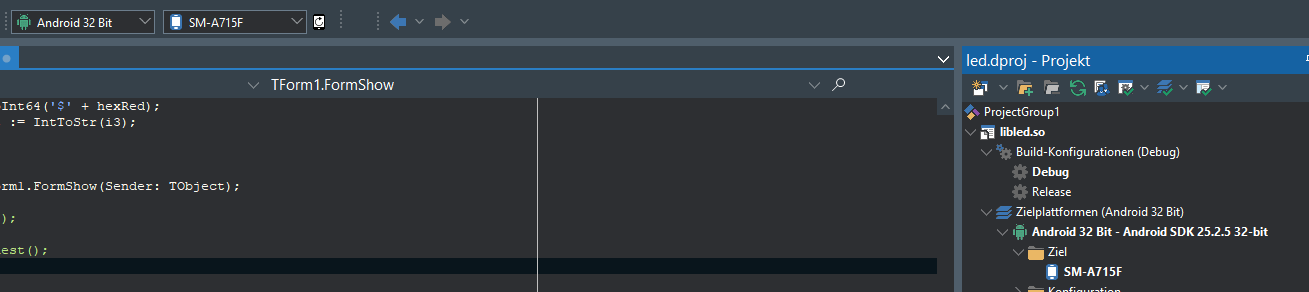
\includegraphics[width=15cm]{img/samsungusb2.png}
\caption{Auswahl des Android Gerätes in der IDE}
\label{samsungusb2}
\end{center}
\end{figure}

\begin{figure}[h]
\begin{center}
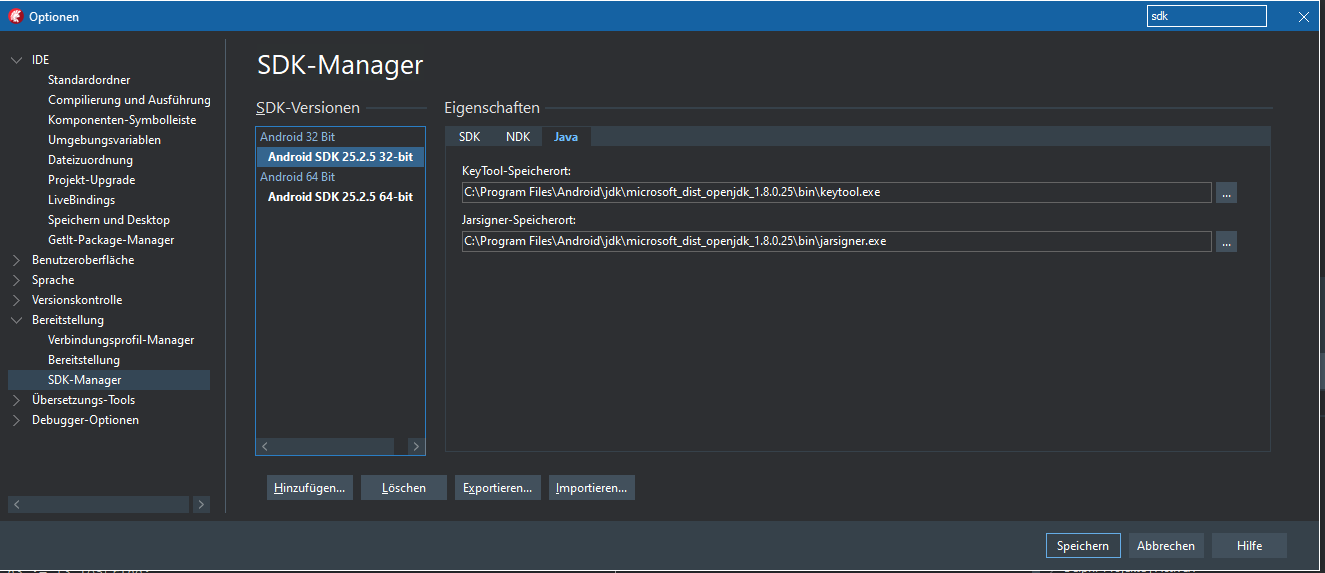
\includegraphics[width=15cm]{img/keytoolexe.png}
\caption{Das richtige Java verwenden}
\label{keytoolexe}
\end{center}
\end{figure}

\begin{figure}[h]
\begin{center}
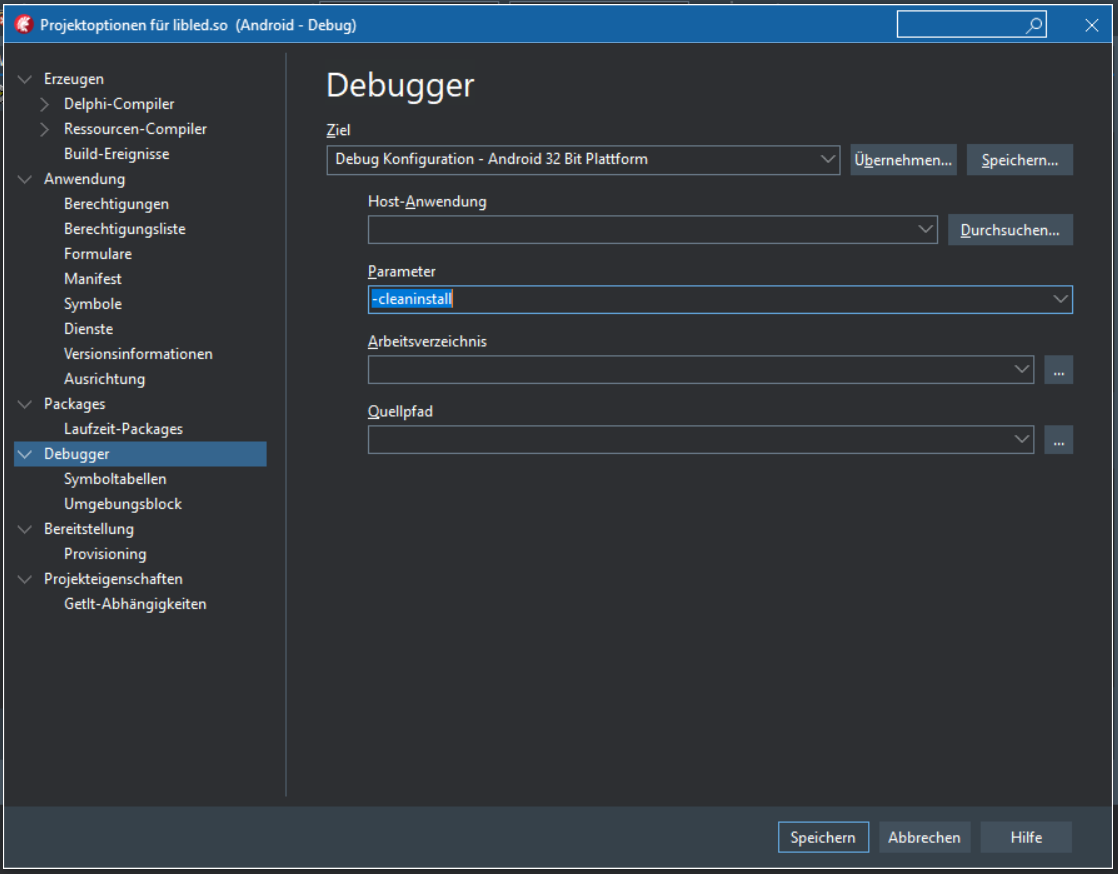
\includegraphics[width=15cm]{img/cleaninstall.png}
\caption{Alle Daten komplett neu mitgeben}
\label{cleaninstall}
\end{center}
\end{figure}

\begin{figure}[h]
\begin{center}
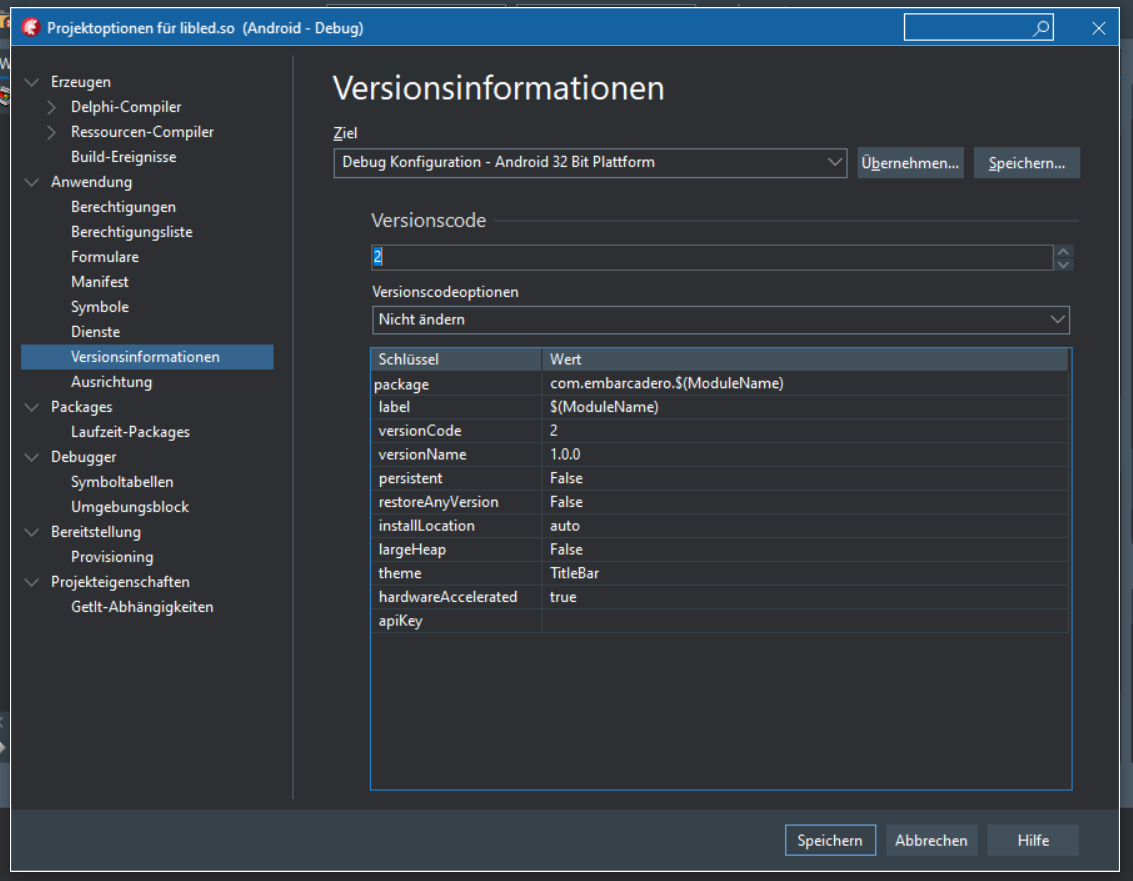
\includegraphics[width=15cm]{img/version.png}
\caption{Version beim kompilieren hoch setzen nach Signatur-Fehler}
\label{version}
\end{center}
\end{figure}

\begin{figure}[h]
\begin{center}
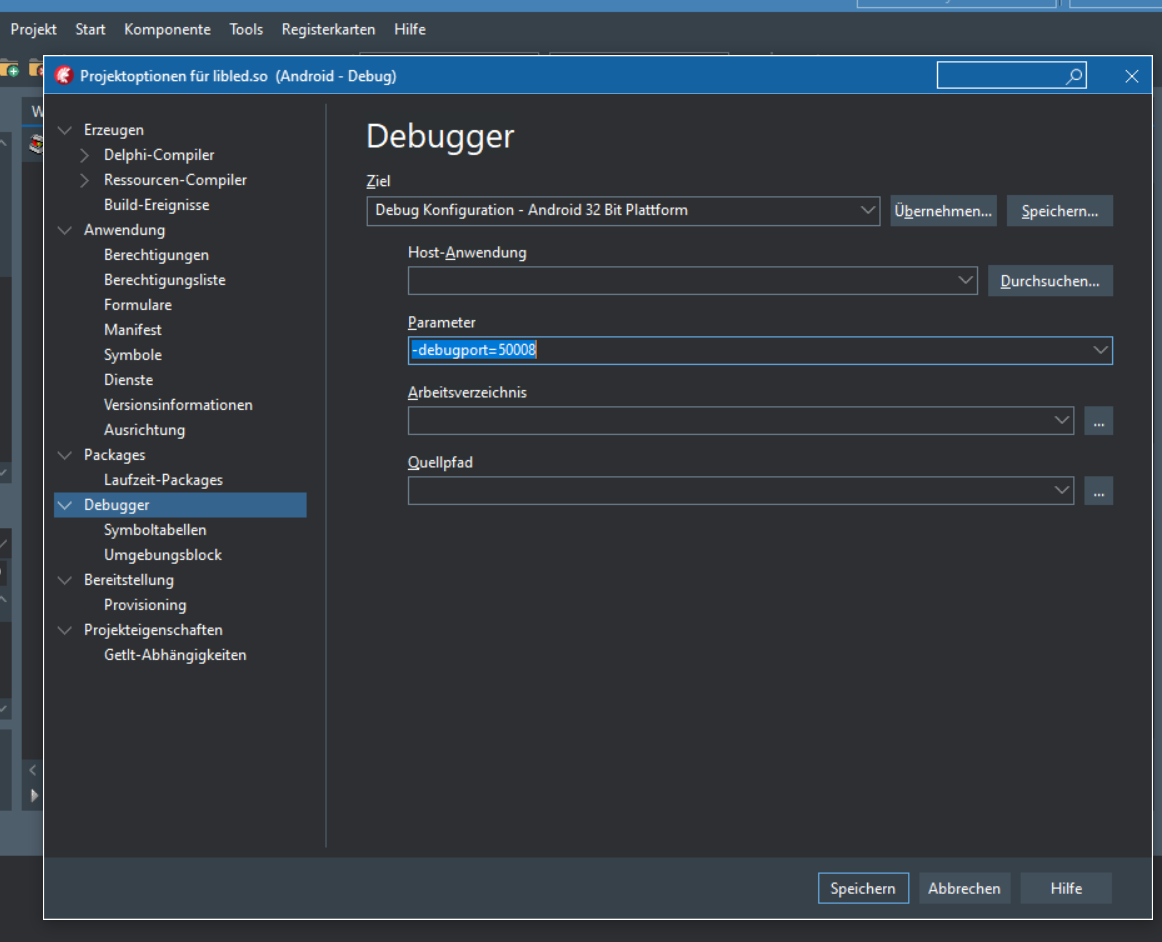
\includegraphics[width=15cm]{img/port.png}
\caption{Den Port ändern nach Signatur Fehler}
\label{port}
\end{center}
\end{figure}

